% answers.tex —— 2022 年·全国乙卷·理科 · 参考答案与详细解析片段
% 由 tools/generate_projects.py 依来源总账自 2022/2022_数学真题_全国乙理_试题.md + 2022/2022_数学真题_全国乙理_解析正文.md + 2022/2022_数学真题_全国乙理_答案要点.md 生成，勿手改（改源 MD 后重跑）


\begin{gktip}
本文只写推导，不复述题面或另立答案源。无官方答案材料；第 11、16 题按源题面问题标 U，其余题目为独立推导并完成盲核（D）。
\end{gktip}

\begin{answer}
\gksolhead{1}{}

\textbf{题目}：

设全集 $U=\{1,2,3,4,5\}$，集合 $M$ 满足 $\complement_U M=\{1,3\}$，则\mbox{（　　）}

\begin{gkopts}(4)
\task A．$2\in M$
\task B．$3\in M$
\task C．$4\notin M$
\task D．$5\notin M$
\end{gkopts}

\begin{gktip}
页码：PDF 第 1 页 / 纸面第 1165 页。
\end{gktip}

\Needspace{4\baselineskip}
\textbf{解析}

$\complement_U M=\{1,3\}$，所以 $M=U\setminus\{1,3\}=\{2,4,5\}$。只有 $2\in M$，选 A。

\gkanswer{答案：A}

\end{answer}
\begin{answer}
\gksolhead{2}{}

\textbf{题目}：

已知 $z=1-2\mathrm i$，且 $z+a\overline z+b=0$，其中 $a,b$ 为实数，则\mbox{（　　）}

\begin{gkopts}(4)
\task A．$a=1,b=-2$
\task B．$a=-1,b=2$
\task C．$a=1,b=2$
\task D．$a=-1,b=-2$
\end{gkopts}

\begin{gktip}
页码：PDF 第 1 页 / 纸面第 1165 页。
\end{gktip}

\Needspace{4\baselineskip}
\textbf{解析}

\Needspace{5\baselineskip}
代入 $z=1-2\mathrm i,\overline z=1+2\mathrm i$：
\nopagebreak[4]
\[
(1-2\mathrm i)+a(1+2\mathrm i)+b=0.
\]
虚部给 $2(a-1)=0$，故 $a=1$；实部给 $1+a+b=0$，故 $b=-2$，选 A。

\gkanswer{答案：A}

\end{answer}
\begin{answer}
\gksolhead{3}{}

\textbf{题目}：

已知向量 $\boldsymbol a,\boldsymbol b$ 满足 $|\boldsymbol a|=1$，$|\boldsymbol b|=\sqrt3$，$|\boldsymbol a-2\boldsymbol b|=3$，则 $\boldsymbol a\cdot\boldsymbol b=$\mbox{（　　）}

\begin{gkopts}(4)
\task A．$-2$
\task B．$-1$
\task C．$1$
\task D．$2$
\end{gkopts}

\begin{gktip}
页码：PDF 第 1 页 / 纸面第 1165 页。
\end{gktip}

\Needspace{4\baselineskip}
\textbf{解析}

\Needspace{5\baselineskip}
两边平方：
\nopagebreak[4]
\[
9=|\boldsymbol a|^2+4|\boldsymbol b|^2-4\boldsymbol a\cdot\boldsymbol b
=1+12-4\boldsymbol a\cdot\boldsymbol b,
\]
所以 $\boldsymbol a\cdot\boldsymbol b=1$，选 C。

\gkanswer{答案：C}

\end{answer}
\begin{answer}
\gksolhead{4}{}

\textbf{题目}：

\Needspace{5\baselineskip}
嫦娥二号卫星在完成探月任务后，继续进行深空探测，成为我国第一颗环绕太阳飞行的人造行星。为研究嫦娥二号绕日周期与地球绕日周期的比值，用到数列 $\{b_n\}$：
\nopagebreak[4]
\[
b_1=1+\frac1{\alpha_1},\quad
b_2=1+\frac1{\alpha_1+\frac1{\alpha_2}},\quad
b_3=1+\frac1{\alpha_1+\frac1{\alpha_2+\frac1{\alpha_3}}},\quad\cdots,
\]
依此类推，其中 $\alpha_k\in\mathbf N^*$（$k=1,2,\ldots$）。则\mbox{（　　）}

\begin{gkopts}(4)
\task A．$b_1<b_5$
\task B．$b_3<b_8$
\task C．$b_6<b_2$
\task D．$b_4<b_7$
\end{gkopts}

\begin{gktip}
页码：PDF 第 1 页 / 纸面第 1165 页。
\end{gktip}

\Needspace{4\baselineskip}
\textbf{解析}

这是正整数部分商的有限连分数截断。增加一层时，外层映射 $x\mapsto1/(\alpha+x)$ 严格递减，故截断值相对极限上下交替；同奇偶子列分别单调。于是奇数项在偶数项一侧，四个比较中只有 $b_4<b_7$ 成立，选 D。

\gkanswer{答案：D}

\end{answer}
\begin{answer}
\gksolhead{5}{}

\textbf{题目}：

设 $F$ 为抛物线 $C:y^2=4x$ 的焦点，点 $A$ 在 $C$ 上，点 $B(3,0)$。若 $|AF|=|BF|$，则 $|AB|=$\mbox{（　　）}

\begin{gkopts}(4)
\task A．$2$
\task B．$2\sqrt2$
\task C．$3$
\task D．$3\sqrt2$
\end{gkopts}

\begin{gktip}
页码：PDF 第 1 页 / 纸面第 1165 页。
\end{gktip}

\Needspace{4\baselineskip}
\textbf{解析}

\Needspace{5\baselineskip}
抛物线焦点为 $F(1,0)$，$|BF|=2$。抛物线上的焦半径满足 $|AF|=x_A+1$，故 $x_A=1$，再由 $y_A^2=4x_A$ 得 $y_A=\pm2$。因此
\nopagebreak[4]
\[
|AB|=\sqrt{(1-3)^2+(\pm2)^2}=2\sqrt2.
\]
选 B。

\gkanswer{答案：B（$2\sqrt2$）}

\end{answer}
\begin{answer}
\gksolhead{6}{}

\textbf{题目}：

执行如图的程序框图，输出的 $n=$\mbox{（　　）}

\begin{gktip}
图示说明：程序框图依次输入 $a=1,b=1,n=1$；循环执行 $b=b+2a$、$a=b-a,n=n+1$；判断 $\left|\dfrac{b^2}{a^2}-2\right|<0.01$，满足时输出 $n$，否则返回循环。
\end{gktip}
\nopagebreak[4]
\begin{center}\begin{tikzpicture}[x=1cm,y=1cm,>=stealth,thick,font=\small]
  % Start
  \draw[rounded corners] (-0.65,0.25) rectangle (0.65,0.95);
  \node at (0,0.6) {开始};
  \draw[->] (0,0.25) -- (0,-0.15);

  % Input parallelogram
  \draw (-1.5,-0.15) -- (1.5,-0.15) -- (1.25,-0.85) -- (-1.25,-0.85) -- cycle;
  \node at (0,-0.5) {输入 $a=1,b=1,n=1$};
  \draw[->] (0,-0.85) -- (0,-1.25);

  % Loop body
  \draw (-1.1,-1.25) rectangle (1.1,-1.95);
  \node at (0,-1.6) {$b=b+2a$};
  \draw[->] (0,-1.95) -- (0,-2.25);
  \draw (-1.45,-2.25) rectangle (1.45,-3.05);
  \node[align=center] at (0,-2.65) {$a=b-a$\\$n=n+1$};
  \draw[->] (0,-3.05) -- (0,-3.45);

  % Decision diamond
  \draw (0,-4.25) -- (2,-3.75) -- (0,-3.25) -- (-2,-3.75) -- cycle;
  \node[align=center] at (0,-3.75) {$\left|\dfrac{b^2}{a^2}-2\right|<0.01$};

  % Yes: output and end
  \draw[->] (0,-4.25) -- (0,-4.65);
  \node at (0.35,-4.48) {是};
  \draw (-1.0,-4.65) -- (1.0,-4.65) -- (0.8,-5.25) -- (-0.8,-5.25) -- cycle;
  \node at (0,-4.95) {输出 $n$};
  \draw[->] (0,-5.25) -- (0,-5.6);
  \draw[rounded corners] (-0.65,-5.6) rectangle (0.65,-6.3);
  \node at (0,-5.95) {结束};

  % No: return to loop body
  \draw[->] (-2,-3.75) -- (-3.0,-3.75) -- (-3.0,-1.6) -- (-1.1,-1.6);
  \node at (-2.45,-3.5) {否};
\end{tikzpicture}
\end{center}
\nopagebreak[4]
\begin{gkopts}(4)
\task A．$3$
\task B．$4$
\task C．$5$
\task D．$6$
\end{gkopts}

\begin{gktip}
页码：PDF 第 1 页 / 纸面第 1165 页。
\end{gktip}

\Needspace{4\baselineskip}
\textbf{解析}

\Needspace{5\baselineskip}
记每次循环前的状态为 $(a,b,n)$。循环依次得到 $(2,3,2)$、$(5,7,3)$、$(12,17,4)$，其中最后一步
\nopagebreak[4]
\[
\left|\frac{17^2}{12^2}-2\right|=\frac1{144}<0.01.
\]
此时输出 $n=4$，选 B。

\gkanswer{答案：B（$n=4$）}

\end{answer}
\begin{answer}
\gksolhead{7}{}

\textbf{题目}：

在正方体 $ABCD-A_1B_1C_1D_1$ 中，$E,F$ 分别为 $AB,BC$ 的中点，则\mbox{（　　）}

\begin{gkopts}(2)
\task A．平面 $B_1EF\perp$ 平面 $BDD_1$
\task B．平面 $B_1EF\perp$ 平面 $A_1BD$
\task C．平面 $B_1EF\parallel$ 平面 $A_1AC$
\task D．平面 $B_1EF\parallel$ 平面 $A_1C_1D$
\end{gkopts}

\begin{gktip}
页码：PDF 第 1 页 / 纸面第 1165 页。
\end{gktip}

\Needspace{4\baselineskip}
\textbf{解析}

设正方体坐标为 $A(0,0,0),B(1,0,0),C(1,1,0),D(0,1,0)$，上层各点的 $z=1$。则 $E=(1/2,0,0),F=(1,1/2,0),B_1=(1,0,1)$，平面 $B_1EF$ 的法向量可取 $(2,-2,-1)$。平面 $BDD_1$ 的法向量可取 $(1,1,0)$，两法向量点积为 $0$，故平面垂直，选 A。

\gkanswer{答案：A}

\end{answer}
\begin{answer}
\gksolhead{8}{}

\textbf{题目}：

已知等比数列 $\{a_n\}$ 的前 3 项和为 $168$，$a_2-a_5=42$，则 $a_6=$\mbox{（　　）}

\begin{gkopts}(4)
\task A．$14$
\task B．$12$
\task C．$6$
\task D．$3$
\end{gkopts}

\begin{gktip}
页码：PDF 第 1 页 / 纸面第 1165 页。
\end{gktip}

\Needspace{4\baselineskip}
\textbf{解析}

\Needspace{5\baselineskip}
设首项为 $u$、公比为 $q$。由
\nopagebreak[4]
\[
u(1+q+q^2)=168,\qquad uq(1-q^3)=42
\]
相除，并用 $1-q^3=(1-q)(1+q+q^2)$，得 $q(1-q)=1/4$，即 $(q-1/2)^2=0$。于是 $q=1/2,u=96$，$a_6=96(1/2)^5=3$，选 D。

\gkanswer{答案：D（$a_6=3$）}

\end{answer}
\begin{answer}
\gksolhead{9}{}

\textbf{题目}：

已知球 $O$ 的半径为 $1$，四棱锥的顶点为 $O$，底面的四个顶点均在球 $O$ 的球面上，则当该四棱锥的体积最大时，其高为\mbox{（　　）}

\begin{gkopts}(2)
\task A．$\dfrac13$
\task B．$\dfrac12$
\task C．$\dfrac{\sqrt3}{3}$
\task D．$\dfrac{\sqrt2}{2}$
\end{gkopts}

\begin{gktip}
页码：PDF 第 1 页 / 纸面第 1165 页。
\end{gktip}

\Needspace{4\baselineskip}
\textbf{解析}

\Needspace{5\baselineskip}
设底面所在平面到球心的距离为 $h$，则底面四点所在截面圆半径为 $r=\sqrt{1-h^2}$。圆内四边形面积至多为内接正方形面积 $2r^2$，故
\nopagebreak[4]
\[
V\le\frac13h\cdot2(1-h^2).
\]
函数 $h(1-h^2)$ 在 $0<h<1$ 的最大值于 $h=1/\sqrt3$ 取得；正方形底面可达到面积上界，故所求高为 $\sqrt3/3$，选 C。

\gkanswer{答案：C}

\end{answer}
\begin{answer}
\gksolhead{10}{}

\textbf{题目}：

某棋手与甲、乙、丙三位棋手各比赛一盘，各盘比赛结果相互独立。已知该棋手与甲、乙、丙比赛获胜的概率分别为 $p_1,p_2,p_3$，且 $p_3>p_2>p_1>0$。记该棋手连胜两盘的概率为 $p$，则\mbox{（　　）}

\begin{gkopts}(2)
\task A．$p$ 与该棋手和甲、乙、丙的比赛次序无关
\task B．该棋手在第二盘与甲比赛，$p$ 最大
\task C．该棋手在第二盘与乙比赛，$p$ 最大
\task D．该棋手在第二盘与丙比赛，$p$ 最大
\end{gkopts}

\begin{gktip}
页码：PDF 第 1 页 / 纸面第 1165 页。
\end{gktip}

\Needspace{4\baselineskip}
\textbf{解析}

\Needspace{5\baselineskip}
若第二盘对手的胜率为 $p_j$，其余两盘胜率为 $p_i,p_k$，则“两盘连胜”为第一、二盘连胜或第二、三盘连胜，扣除三盘全胜的重叠：
\nopagebreak[4]
\[
p=p_ip_j+p_jp_k-p_ip_jp_k=p_j(p_i+p_k-p_ip_k).
\]
将 $p_1,p_2,p_3$ 分别作为中间项比较。以 $p_3$ 为中间项比以 $p_2$ 为中间项多 $p_1(p_3-p_2)>0$；比以 $p_1$ 为中间项多 $p_2(p_3-p_1)>0$。故第二盘与丙比赛时概率最大，选 D。

\gkanswer{答案：D}

\end{answer}
\begin{answer}
\gksolhead{11}{}

\textbf{题目}：

双曲线 $C$ 的两个焦点为 $F_1,F_2$，以 $C$ 的实轴为直径的圆记为 $D$。过 $F_1$ 作 $D$ 的切线与 $C$ 交于 $M,N$ 两点，且 $\cos\angle F_1NF_2=\dfrac35$，则 $C$ 的离心率为\mbox{（　　）}

\begin{gkopts}(2)
\task A．$\dfrac{\sqrt5}{2}$
\task B．$\dfrac32$
\task C．$\dfrac{\sqrt{13}}2$
\task D．$\dfrac{\sqrt{17}}2$
\end{gkopts}

\begin{gktip}
页码：PDF 第 1 页 / 纸面第 1165 页。
\end{gktip}

\Needspace{4\baselineskip}
\textbf{解析}

题面未规定 $N$ 所在分支或 $M,N$ 的顺序。取半实轴 $a=1$：

\begin{itemize}
\item 选项 A：$e=\sqrt5/2,b=1/2$。直线 $y=2(x-\sqrt5/2)$ 与以实轴为直径的圆相切；双曲线上可取交点 $N=(3\sqrt5/5,\sqrt5/5)$，且 $|NF_1|=1/2,|NF_2|=5/2$，所以 $\cos\angle F_1NF_2=3/5$。
\item 选项 C：$e=\sqrt{13}/2,b=3/2$。直线 $y=\frac23(x-\sqrt{13}/2)$ 也与该圆相切；双曲线上可取 $N=(-7/\sqrt{13},-9/\sqrt{13})$，且两焦点距离为 $9/2,5/2$，余弦同样为 $3/5$。
\end{itemize}

因此至少有 A、C 两个选项符合当前题面，不能据此唯一确定答案。

\gkanswer{答案：U/PENDING；题面未指定 $N$ 的分支或 $M,N$ 的顺序，A、C 两个选项均可由满足条件的构造得到}

\end{answer}
\begin{answer}
\gksolhead{12}{}

\textbf{题目}：

已知函数 $f(x),g(x)$ 的定义域均为 $\mathbf R$，且 $f(x)+g(2-x)=5$，$g(x)-f(x-4)=7$。若 $y=g(x)$ 的图象关于直线 $x=2$ 对称，$g(2)=4$，则 $\displaystyle\sum_{k=1}^{22}f(k)=$\mbox{（　　）}

\begin{gkopts}(4)
\task A．$-21$
\task B．$-22$
\task C．$-23$
\task D．$-24$
\end{gkopts}

\begin{gktip}
页码：PDF 第 1 页 / 纸面第 1165 页。
\end{gktip}

\Needspace{4\baselineskip}
\textbf{解析}

\Needspace{5\baselineskip}
$g$ 关于 $x=2$ 对称即 $g(4-x)=g(x)$。由 $f(x)+g(2-x)=5$ 得 $f(x)=5-g(2+x)$；代入第二个关系并用对称性可得
\nopagebreak[4]
\[
g(x)+g(x-2)=12.
\]
再由 $g(2)=4$ 得偶整数点值按 $g(4j)=8,g(4j+2)=4$ 交替，奇整数点值为 $6$。因为 $f(k)=5-g(k+2)$，$k=1,\ldots,22$ 对应 $g(3),\ldots,g(24)$。其中 11 个奇数点合计 $66$；偶数点中 6 个值为 $8$、5 个值为 $4$，合计 $68$。因此 $\sum f(k)=22\cdot5-(66+68)=-24$，选 D。

\gkanswer{答案：D（求和为 $-24$）}

\end{answer}
\begin{answer}
\gksolhead{13}{}

\textbf{题目}：

从甲、乙等 5 名同学中随机选 3 名参加社区服务工作，则甲、乙都入选的概率为 \gkblank{}。

\begin{gktip}
页码：PDF 第 1 页 / 纸面第 1165 页。
\end{gktip}

\Needspace{4\baselineskip}
\textbf{解析}

从 5 人中选 3 人共有 $\binom53=10$ 种；固定甲、乙入选后，第三人从其余 3 人中选，故概率为 $3/10$。

\gkanswer{答案：$3/10$}

\end{answer}
\begin{answer}
\gksolhead{14}{}

\textbf{题目}：

过四点 $(0,0),(4,0),(-1,1),(4,2)$ 中的三点的一个圆的方程为 \gkblank{}。

\begin{gktip}
页码：PDF 第 1 页 / 纸面第 1165 页。
\end{gktip}

\Needspace{4\baselineskip}
\textbf{解析}

选取 $(0,0),(4,0),(4,2)$。前两点的垂直平分线为 $x=2$；与第三点等距给圆心 $(2,1)$，半径平方为 $5$。方程为 $(x-2)^2+(y-1)^2=5$，即 $x^2+y^2-4x-2y=0$。

\gkanswer{答案：$x^2+y^2-4x-2y=0$（一个有效例子）}

\end{answer}
\begin{answer}
\gksolhead{15}{}

\textbf{题目}：

记函数 $f(x)=\cos(\omega x+\varphi)$（$\omega>0,0<\varphi<\pi$）的最小正周期为 $T$。若 $f(T)=\dfrac{\sqrt3}{2}$，$x=\dfrac\pi9$ 为 $f(x)$ 的零点，则 $\omega$ 的最小值为 \gkblank{}。

\begin{gktip}
页码：PDF 第 1 页 / 纸面第 1165 页。
\end{gktip}

\Needspace{4\baselineskip}
\textbf{解析}

\Needspace{5\baselineskip}
$f(T)=\cos(\omega T+\varphi)=\cos\varphi=\sqrt3/2$，由 $0<\varphi<\pi$ 得 $\varphi=\pi/6$。零点条件要求
\nopagebreak[4]
\[
\omega\frac\pi9+\frac\pi6=\frac\pi2+k\pi,
\]
即 $\omega=3+9k$。最小正值取 $k=0$，为 $3$。

\gkanswer{答案：$3$}

\end{answer}
\begin{answer}
\gksolhead{16}{}

\textbf{题目}：

已知 $x=x_1$ 和 $x=x_2$ 分别是函数 $f(x)=2a^x-e^{x^2}$（$a>0$ 且 $a\ne1$）的极小值点和极大值点。若 $x_1<x_2$，则 $a$ 的取值范围是 \gkblank{}。

\begin{gktip}
页码：PDF 第 1 页 / 纸面第 1165 页。
\end{gktip}

\Needspace{4\baselineskip}
\textbf{解析}

\Needspace{5\baselineskip}
原卷函数为 $f(x)=2a^x-e^{x^2}$，$a>0,a\ne1$。若 $a>1$，令 $c=\ln a>0$。$f'(x)>0$ 对 $x\le0$；对 $x>0$，导数符号等于
\nopagebreak[4]
\[
H(x)=\ln(c/x)+cx-x^2.
\]
令 $r=x/c$，则 $H=-\ln r+c^2r(1-r)$，所以 $x<c$ 时 $H>0$，$x>c$ 时 $H<0$。因此唯一驻点为 $x=c$，且为极大值点。若 $0<a<1$，令 $c=-\ln a>0$。此时 $f'(x)<0$ 对 $x\ge0$；对 $x<0$ 令 $t=-x$，导数符号等于 $-H(t)$，故唯一驻点为 $x=-c$，同样为极大值点。又 $f(x)\to-\infty$ 当 $x\to\pm\infty$，故函数没有极小值点。题干同时要求极小值点 $x_1$ 与极大值点 $x_2$，与原式矛盾；保留原题，不猜填空答案。

\gkanswer{答案：U/PENDING；原式对题设范围内的 $a$ 只有一个极大值点，没有极小值点}

\end{answer}
\begin{answer}
\gksolhead{17}{}

\textbf{题目}：

\Needspace{5\baselineskip}
记 $\triangle ABC$ 的内角 $A,B,C$ 的对边分别为 $a,b,c$，已知
\nopagebreak[4]
\[
\sin C\sin(A-B)=\sin B\sin(C-A).
\]

  (1) 证明：$2a^2=b^2+c^2$；

  (2) 若 $a=5,\cos A=\dfrac{25}{31}$，求 $\triangle ABC$ 的周长。

\begin{gktip}
页码：PDF 第 1 页 / 纸面第 1165 页。
\end{gktip}

\Needspace{4\baselineskip}
\textbf{解析}

\textbf{(1) 证明}

\Needspace{5\baselineskip}
展开题设等式并移项整理：
\nopagebreak[4]
\[
\sin A[\sin C\cos B+\sin B\cos C]=2\sin B\sin C\cos A.
\]
括号为 $\sin(B+C)=\sin A$，故 $\sin^2A=2\sin B\sin C\cos A$。用正弦定理化为 $a^2=2bc\cos A$，再代入余弦定理 $2bc\cos A=b^2+c^2-a^2$，即 $2a^2=b^2+c^2$。

\textbf{(2) 解}

当 $a=5,\cos A=25/31$ 时，$b^2+c^2=50$；余弦定理给 $25=50-2bc(25/31)$，所以 $bc=31/2$。于是 $(b+c)^2=50+31=81$，周长 $a+b+c=14$。

\gkanswer{答案（1）：$2a^2=b^2+c^2$}

\gkanswer{答案（2）：周长 $14$}

\end{answer}
\begin{answer}
\gksolhead{18}{}

\textbf{题目}：

如图，四面体 $ABCD$ 中，$AD\perp CD$，$AD=CD$，$\angle ADB=\angle BDC$，$E$ 为 $AC$ 的中点。

  (1) 证明：平面 $BED\perp$ 平面 $ACD$；

  (2) 设 $AB=BD=2,\angle ACB=60^\circ$，点 $F$ 在 $BD$ 上，当 $\triangle AFC$ 的面积最小时，求 $CF$ 与平面 $ABD$ 所成的角的正弦值。

\begin{gktip}
图示说明：按源卷四面体示意独立重绘（非按比例）。
\end{gktip}
\nopagebreak[4]
\begin{center}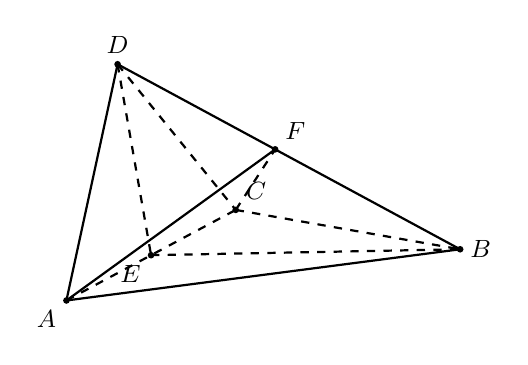
\begin{tikzpicture}[x=1cm,y=1cm,thick,font=\small]
  % Schematic projection only; not to scale.
  \coordinate (A) at (0,0);
  \coordinate (D) at (0.65,3.0);
  \coordinate (B) at (5.0,0.65);
  \coordinate (C) at (2.15,1.15);
  \coordinate (E) at (1.075,0.575);
  \coordinate (F) at (2.651,1.919);

  % Visible outline
  \draw (A)--(D)--(B)--(A);
  % Hidden/interior edges in the source schematic
  \draw[dashed] (A)--(C);
  \draw (A)--(F);
  \draw[dashed] (D)--(C);
  \draw[dashed] (C)--(B);
  \draw[dashed] (D)--(E);
  \draw[dashed] (E)--(B);
  % Segment CF is shown for the queried line-plane angle
  \draw[dashed] (C)--(F);

  \fill (A) circle (1.2pt) node[below left] {$A$};
  \fill (B) circle (1.2pt) node[right] {$B$};
  \fill (C) circle (1.2pt) node[above right] {$C$};
  \fill (D) circle (1.2pt) node[above] {$D$};
  \fill (E) circle (1.2pt) node[below left] {$E$};
  \fill (F) circle (1.2pt) node[above right] {$F$};
\end{tikzpicture}
\end{center}
\nopagebreak[4]
\begin{gktip}

页码：PDF 第 1 页 / 纸面第 1165 页。
\end{gktip}

\Needspace{4\baselineskip}
\textbf{解析}

\textbf{(1) 证明}

取 $D=(0,0,0),A=(s,0,0),C=(0,s,0)$，其中 $s=AD=CD$。由 $\angle ADB=\angle BDC$ 和 $AD=CD$，可知 $B$ 到 $DA,DC$ 两方向的夹角相等，故可写 $B=(u,u,v)$。$DE$ 的方向为 $(1,1,0)$，$DB=(u,u,v)$ 也在平面 $x=y$ 内，且 $E=(s/2,s/2,0)$。因此平面 $BED$ 就是 $x=y$，其法向量平行 $(1,-1,0)$，与平面 $ACD$ 的法向量 $(0,0,1)$ 垂直，故两平面垂直。

\textbf{(2) 解}

\Needspace{5\baselineskip}
$AB=BD$ 给 $u=s/2$。由 $BD=2$ 得 $s^2/2+v^2=4$；又
\nopagebreak[4]
\[
\cos\angle ACB=\frac{\overrightarrow{CA}\cdot\overrightarrow{CB}}{|CA||CB|}
=\frac{s}{2\sqrt2}=\frac12,
\]
故 $s=\sqrt2,v^2=3$。令 $F=tB$（$0\le t\le1$）。点 $F$ 到直线 $AC$ 的距离平方为 $(1-t)^2+3t^2$，因此 $[AFC]$ 最小时 $t=1/4$。

\Needspace{5\baselineskip}
取 $v=\sqrt3$（取负号不影响正弦），则
\nopagebreak[4]
\[
A=(\sqrt2,0,0),\ B=(\tfrac1{\sqrt2},\tfrac1{\sqrt2},\sqrt3),\
C=(0,\sqrt2,0),\ F=(\tfrac{\sqrt2}8,\tfrac{\sqrt2}8,\tfrac{\sqrt3}4).
\]
\Needspace{5\baselineskip}
平面 $ABD$ 的法向量可取 $\boldsymbol n=(0,-\sqrt6,1)$，$|\boldsymbol n|=\sqrt7$；$\overrightarrow{CF}\cdot\boldsymbol n=2\sqrt3$，$|CF|=\sqrt7/2$。线面角 $\theta$ 满足
\nopagebreak[4]
\[
\sin\theta=\frac{|\overrightarrow{CF}\cdot\boldsymbol n|}{|CF||\boldsymbol n|}=\frac{4\sqrt3}{7}.
\]

\gkanswer{答案（1）：见解析版}

\gkanswer{答案（2）：$\dfrac{4\sqrt3}{7}$}

\end{answer}
\begin{answer}
\gksolhead{19}{}

\textbf{题目}：

某地经过多年的环境治理，已将荒山改造成了绿水青山。为估计一林区某种树木的总材积量，随机选取了 10 棵这种树木，测量每棵树的根部横截面积（单位：$\mathrm m^2$）和材积量（单位：$\mathrm m^3$），得到下表：

\begin{center}
\begingroup\setlength{\tabcolsep}{4pt}
\begin{tabular}{lrrrrrrrrrrr}
\toprule
样本号 $i$ & 1 & 2 & 3 & 4 & 5 & 6 & 7 & 8 & 9 & 10 & 总和 \\
\midrule
根部横截面积 $x_i$ & 0.04 & 0.06 & 0.04 & 0.08 & 0.08 & 0.05 & 0.05 & 0.07 & 0.07 & 0.06 & 0.6 \\
材积量 $y_i$ & 0.25 & 0.40 & 0.22 & 0.54 & 0.51 & 0.34 & 0.36 & 0.46 & 0.42 & 0.40 & 3.9 \\
\bottomrule
\end{tabular}
\endgroup
\end{center}

并计算得 $\displaystyle\sum_{i=1}^{10}x_i^2=0.038$，$\displaystyle\sum_{i=1}^{10}y_i^2=1.6158$，$\displaystyle\sum_{i=1}^{10}x_iy_i=0.2474$。

  (1) 估计该林区这种树木平均一棵的根部横截面积与平均一棵的材积量；

  (2) 求该林区这种树木的根部横截面积与材积量的样本相关系数（精确到 $0.01$）；

  (3) 现测量了该林区所有这种树木的根部横截面积，并得到所有这种树木的根部横截面积总和为 $186\ \mathrm m^2$。已知树木的材积量与其根部横截面积近似成正比。利用以上数据给出该林区这种树木的总材积量的估计值。

附：$\displaystyle r=\frac{\sum_{i=1}^n(x_i-\bar x)(y_i-\bar y)}{\sqrt{\sum_{i=1}^n(x_i-\bar x)^2\sum_{i=1}^n(y_i-\bar y)^2}}$，$\sqrt{1.896}\approx1.377$。

\begin{gktip}
页码：PDF 第 2 页 / 纸面第 1166 页。
\end{gktip}

\Needspace{4\baselineskip}
\textbf{解析}

\textbf{(1) 解}

$\bar x=0.6/10=0.06\ \mathrm m^2$，$\bar y=3.9/10=0.39\ \mathrm m^3$。

\textbf{(2) 解}

\Needspace{5\baselineskip}
中心化平方和为
\nopagebreak[4]
\[
S_{xx}=0.038-10(0.06)^2=0.002,\quad
S_{yy}=1.6158-10(0.39)^2=0.0948,
\]
\Needspace{5\baselineskip}
中心化乘积和 $S_{xy}=0.2474-10(0.06)(0.39)=0.0134$。故
\nopagebreak[4]
\[
r=\frac{0.0134}{\sqrt{0.002\cdot0.0948}}
=\frac{0.0134}{0.01\sqrt{1.896}}\approx0.973\approx0.97.
\]
\textbf{(3) 解}

材积量与面积近似成正比，单位面积估计系数为 $0.39/0.06=6.5\ \mathrm m$，所以总材积量估计 $186\ \mathrm m^2\times6.5\ \mathrm m=1209\ \mathrm m^3$，量纲为体积。

\gkanswer{答案（1）：$0.06\ \mathrm m^2,\ 0.39\ \mathrm m^3$}

\gkanswer{答案（2）：$r=0.97$}

\gkanswer{答案（3）：$1209\ \mathrm m^3$}

\end{answer}
\begin{answer}
\gksolhead{20}{}

\textbf{题目}：

已知椭圆 $E$ 的中心为坐标原点，对称轴为 $x$ 轴、$y$ 轴，且过 $A(0,-2),B\left(\dfrac32,-1\right)$ 两点。

  (1) 求 $E$ 的方程；

  (2) 设过点 $P(1,-2)$ 的直线交 $E$ 于 $M,N$ 两点，过 $M$ 且平行于 $x$ 轴的直线与线段 $AB$ 交于点 $T$，点 $H$ 满足 $\overrightarrow{MT}=\overrightarrow{TH}$。证明：直线 $HN$ 过定点。

\begin{gktip}
页码：PDF 第 2 页 / 纸面第 1166 页。
\end{gktip}

\Needspace{4\baselineskip}
\textbf{解析}

\textbf{(1) 解}

椭圆方程写作 $x^2/a^2+y^2/b^2=1$。由 $A(0,-2)$ 得 $b^2=4$；代入 $B(3/2,-1)$ 得 $9/(4a^2)+1/4=1$，故 $a^2=3$。

\textbf{(2) 解}

\Needspace{5\baselineskip}
设过 $P$ 的非竖直直线参数式为 $(x,y)=(1+t,-2+kt)$，与椭圆交于参数 $\lambda,\mu$。代入方程得
\nopagebreak[4]
\[
\left(\frac13+\frac{k^2}4\right)t^2+\left(\frac23-k\right)t+\frac13=0.
\]
\Needspace{5\baselineskip}
记 $D=1/3+k^2/4$，则 $\lambda+\mu=(k-2/3)/D$、$\lambda\mu=1/(3D)$。令 $M$ 对应 $\lambda$、$N$ 对应 $\mu$。$T$ 在 $AB$ 且与 $M$ 同高，故 $T=(3k\lambda/2,-2+k\lambda)$；由 $\overrightarrow{MT}=\overrightarrow{TH}$，得 $H=(-1+(3k-1)\lambda,-2+k\lambda)$。检验 $A=(0,-2),N,H$ 共线，其行列式化简为
\nopagebreak[4]
\[
(A-N)\times(H-N)=k\bigl[-(\lambda+\mu)+(3k-2)\lambda\mu\bigr]=0,
\]
因为 $\lambda+\mu=(k-2/3)/D=(3k-2)/(3D)=(3k-2)\lambda\mu$。故直线 $HN$ 恒过 $A(0,-2)$。竖直线情形由连续性或直接代入可得同一结论。

\gkanswer{答案（1）：$\dfrac{x^2}{3}+\dfrac{y^2}{4}=1$}

\gkanswer{答案（2）：定点 $A(0,-2)$}

\end{answer}
\begin{answer}
\gksolhead{21}{}

\textbf{题目}：

已知函数 $f(x)=\ln(1+x)+axe^{-x}$。

  (1) 当 $a=1$ 时，求曲线 $y=f(x)$ 在点 $(0,f(0))$ 处的切线方程；

  (2) 若 $f(x)$ 在区间 $(-1,0),(0,+\infty)$ 各恰有一个零点，求 $a$ 的取值范围。

\begin{gktip}
页码：PDF 第 2 页 / 纸面第 1166 页。
\end{gktip}

\Needspace{4\baselineskip}
\textbf{解析}

\textbf{(1) 解}

$f(0)=0$，且 $f'(x)=1/(1+x)+ae^{-x}(1-x)$，故 $a=1$ 时 $f'(0)=2$，切线为 $y=2x$。

\textbf{(2) 解}

\Needspace{5\baselineskip}
对正根 $x>0$，方程 $f(x)=0$ 等价于
\nopagebreak[4]
\[
a=-h_+(x),\qquad h_+(x)=\frac{e^x\ln(1+x)}x.
\]
$h_+$ 严格递增，$h_+(0+)=1,h_+(+\infty)=+\infty$，所以正区间恰有一个零点当且仅当 $a<-1$。

对负根 $-1<x<0$，同一方程等价于 $-a=h_-(x)=e^x\ln(1+x)/x$。$h_-$ 在该区间从 $+\infty$ 降至唯一极小值后升至 $1$；故水平值大于 $1$ 与其恰交一次。若 $a<-1$，$-a>1$，负区间也恰有一个零点。两条件合并得 $a<-1$。

\gkanswer{答案（1）：$y=2x$}

\gkanswer{答案（2）：$a<-1$}

\end{answer}
\begin{answer}
\gksolhead{22}{}

\textbf{题目}（选考题，二选一）：

\Needspace{5\baselineskip}
在直角坐标系 $xOy$ 中，曲线 $C$ 的参数方程为
\nopagebreak[4]
\[
\begin{cases}
x=\sqrt3\cos 2t,\\
y=2\sin t
\end{cases}
\quad(t\text{ \text{为参数}}).
\]
以坐标原点为极点，$x$ 轴正半轴为极轴建立极坐标系，已知直线 $l$ 的极坐标方程为 $\rho\sin\left(\theta+\dfrac\pi3\right)+m=0$。

  (1) 写出 $l$ 的直角坐标方程；

  (2) 若 $l$ 与 $C$ 有公共点，求 $m$ 的取值范围。

\begin{gktip}
页码：PDF 第 2 页 / 纸面第 1166 页。
\end{gktip}

\Needspace{4\baselineskip}
\textbf{解析}

\textbf{(1) 解}

\Needspace{5\baselineskip}
极坐标到直角坐标用 $\rho\sin\theta=y,\rho\cos\theta=x$：
\nopagebreak[4]
\[
\rho\sin(\theta+\pi/3)+m=0
\iff \frac y2+\frac{\sqrt3x}2+m=0
\iff \sqrt3x+y+2m=0.
\]
\textbf{(2) 解}

代入参数方程，令 $u=\sin t\in[-1,1]$，则 $\sqrt3x+y=3\cos2t+2\sin t=3-6u^2+2u$。该二次函数在 $u=1/6$ 取最大值 $19/6$，端点最小值为 $-5$。存在交点等价于 $-2m\in[-5,19/6]$，故 $m\in[-19/12,5/2]$。

\gkanswer{答案（1）：$\sqrt3x+y+2m=0$}

\gkanswer{答案（2）：$m\in[-19/12,5/2]$}

\end{answer}
\begin{answer}
\gksolhead{23}{}

\textbf{题目}（选考题，二选一）：

已知 $a,b,c$ 都是正数，且 $a^{3/2}+b^{3/2}+c^{3/2}=1$，证明：

  (1) $abc\le\dfrac19$；

  (2) $\displaystyle\frac{a}{b+c}+\frac{b}{a+c}+\frac{c}{a+b}\le\frac1{2\sqrt{abc}}$。

\begin{gktip}
页码：PDF 第 2 页 / 纸面第 1166 页。
\end{gktip}

\Needspace{4\baselineskip}
\textbf{解析}

\textbf{(1) 证明}

令 $x=a^{3/2},y=b^{3/2},z=c^{3/2}$，则 $x+y+z=1$。由 AM-GM，$xyz\le1/27$，所以 $abc=(xyz)^{2/3}\le1/9$。

\textbf{(2) 解}

\Needspace{5\baselineskip}
由 $b+c\ge2\sqrt{bc}$，有
\nopagebreak[4]
\[
\frac a{b+c}\le\frac a{2\sqrt{bc}}
=\frac{a^{3/2}}{2\sqrt{abc}}.
\]
\Needspace{5\baselineskip}
对三项循环求和，并用 $a^{3/2}+b^{3/2}+c^{3/2}=1$，得到
\nopagebreak[4]
\[
\frac a{b+c}+\frac b{a+c}+\frac c{a+b}\le\frac1{2\sqrt{abc}}.
\]

\gkanswer{答案（1）：$abc\le1/9$}

\gkanswer{答案（2）：题设不等式成立，等号在 $a=b=c=3^{-2/3}$ 时取到}

\end{answer}